\section{Implementation}

\subsection{Engine architecture}
The architecture of the engine is mainly focused on the concepts of file loading and parsing, object oriented wrapping of OpenGL, scene objects, and render passes.

\subsubsection{File loading and parsing}
\paragraph{BART}
Benchmark for Animated Raytracing (BART) is a scene description format used to compare ray tracing algorithms. On the BART homepage \cite{bart_homepage}, there are three test scenes designed to stress raytracing algorithms. All the scenes use traditional triangle based geometry. The camera and object animation paths are animated using  Kochanek-Bartels splines. The BART format is an extension of the Eric Haines' natural file format (NFF). The source code available doesn't seem to be maintained and didn't work out of the box, so we had to patch it up and make it work with both GL buffer objects (GLBO) and OptiX. We did not find the time to implement animations.

\paragraph{Assimp}
The Assimp homepage \cite{assimp_homepage} defines the library like this:
\begin{Verbatim}[frame=single,fontshape=it,framesep=1mm]
Open Asset Import Library (short name: Assimp) is a portable
Open Source library to import various well-known 3D model formats
in a uniform manner. The most recent version also knows how to 
export  3d files and is therefore suitable as general-purpose 
3D model converter.
\end{Verbatim}

In our engine, we use Assimp to load 3d model files generated in 3rd party polygon-based modelling software, and parse them into triangle-based buffers that is uploaded to hardware buffers with OpenGL. The engine can also convert this data to buffers for use in OptiX.

\paragraph{Shaders}
Shaders are loaded from files using the old fopen from \textless stdio.h\textgreater . The shader loader also has a shader binding stack, for convenience, allowing render passes and scene objects to push and pop shaders' active state.
The state of each shader is contained in the Shader object. It's implementation is based on the program pipeline API in OpenGL 4.

\paragraph{Textures}
The texture loader is based on DevIL, who's homepage \cite{devil_homepage} describes the library like this:
\begin{Verbatim}[frame=single,fontshape=it,framesep=1mm]
Developer's Image Library (DevIL), formerly known as OpenIL, 
is a programmer's library to  develop applications with very
powerful image loading capabilities, yet is easy for a developer
to learn and use. Ultimate control of images is left to the 
developer, so unnecessary conversions, etc. are not performed.
DevIL utilizes a simple yet powerful syntax. 

DevIL can load, save, convert, manipulate, filter and display a 
wide variety of image formats.
\end{Verbatim}

The texture loader in our engine loads a Tex2D object instance, which wraps the texture handling mechanisms in OpenGL for 2D textures.

\paragraph{Materials}
Materials say something about the basic material properties of the objects they're associated with, with settings such as ambient, diffuse, specular, phong power, transparency and index of refraction.

The implementation is based on an INI parser, which loads the information into a Material object. The Material object contains a Uniform for each property, making it easy to expose it's settings to a bound shader.

\paragraph{Configuration}
The configuration files are simple INI files specialized for a specific purpose in the engine. We have an engine.ini and a scene.ini file for configuring the engine and the scene.

The engine.ini is loaded by the Kernel, and is used to define the screen properties, logic update rate and opengl runtime version.

The scene.ini is loaded by the SceneManager, and is used to define which BART scene to load.

\subsubsection{Object oriented OpenGL wrappers}
As was explained in chapter (about OpenGL), the OpenGL API is a stack-based state machine. In an engine architecture, it makes for more robust handling when a certain behavior is grouped or stored within a class, and take advantage of the construction of objects and destruction of objects, to automate the state of the OpenGL stack as much as possible.

\lstset{language=C++,caption={VBO header},label=vbo.h}
\begin{lstlisting}
class VBO //Vertex Buffer Object
{
	public:
	VBO(unsigned int size, unsigned int draw_type)
	{
		glGenBuffers(1, &handle);
		bind();
		glBufferData(GL_ARRAY_BUFFER, size, nullptr, 
		             draw_type);
	}
	
	~VBO() { glDeleteBuffers(1, &handle); }
	
	void bind()
	{
		glBindBuffer(GL_ARRAY_BUFFER, handle);
		offset = 0;
	}
	void unbind() { glBindBuffer(GL_ARRAY_BUFFER, 0); }
	unsigned int getHandle() const { return handle; }
	
	template<class T>
	unsigned int buffer(const std::vector<T> &data)
	{
		glBufferSubData(GL_ARRAY_BUFFER, offset, 
										sizeof(T)*data.size(), &data[0]);
		unsigned int return_offset = offset;
		offset += sizeof(T)*data.size();
		return return_offset;
	}
	private:
	unsigned int handle;
	unsigned int offset;
};
\end{lstlisting}

\subsubsection{Scene objects}

The scene consist of multiple graphical objects positioned on the screen, and scene objects represents these by declaring the OpenGL render buffers, etc...

\lstset{language=C++,caption={Fullscreen quad implementation},label=quad.cpp}
\begin{lstlisting}
#include "Quad.h"
#include "../Render/ATTRIB.h"
#include "../Render/ShaderConstants.h"
#include <vector>

using namespace std;

Quad::Quad()
{
   unsigned int indices[] = {0,1,2, 2,3,0}; //6
   const float s = 1.0f;
   float vertices[] = {-s,-s, +s,-s, +s,+s, -s,+s}; //8

   unsigned int buffer_size = sizeof(float) * 8;

   vao = make_shared<VAO>();
   vbo = make_shared<VBO>(buffer_size, GL_STATIC_DRAW);
   ibo = make_shared<IBO>(vector<unsignedint>(indices,indices+6),
                          GL_STATIC_DRAW);

   auto v_offset = vbo->buffer<float>(vector<float>(vertices, 
                                                    vertices+8));

   ATTRIB::bind(ShaderConstants::Position(), 2, GL_FLOAT, false, 
                0, v_offset);

   vao->unbind();
   vbo->unbind();
   ibo->unbind();
}

void Quad::render()
{
   vao->bind();
   glDrawElements(GL_TRIANGLES, ibo->size(), GL_UNSIGNED_INT, 
                  BUFFER_OFFSET(0));
}
\end{lstlisting}

\subsubsection{Render pass}
A render pass defines a group of scene objects to be rendered by the rasterizer or raytracer, and can write to render buffers or the back buffer. The SceneManager object defines the order in which the different passes are called, and often one render pass depends on another in order to move down the render pipeline. For instance, the final light pass requires that at least the g-buffer pass has been made in order to work.

\lstset{language=C++,caption={Scene Manager's render implementation},label=scenemanager.cpp}
\begin{lstlisting}
void SceneManager::render()
{
   g_buffer_pass->begin();
   {
      for(auto it = begin(scene); it!=end(scene); ++it )
         (*it)->render(g_buffer_pass->getShader());
   } g_buffer_pass->end();

   raytrace_pass->begin();
   {
      raytrace_pass->render();
   } raytrace_pass->end();

   final_pass->begin();
   {
      bindLights(final_pass->getShader());
      final_pass->render();
   } final_pass->end();
}
\end{lstlisting}

\subsection{Deferred pipeline}
The pipeline of the deferred renderer is broken up into two render passes. The G-buffer pass and the final light pass.

\subsubsection{G-buffer pass}
In the G-buffer pass, all geometry in the scene is rendered by the rasterizer. Position, diffuse and normal data is stored in an MRT in view space.

\lstset{language=C++,caption={G-buffer vertex shader},label=gbuffer.vert}
\begin{lstlisting}
#version 330 core
#define DIFFUSE  0
#define POSITION 1
#define NORMAL   2
#define TEXCOORD 3

uniform mat4 Object_to_World;
uniform mat4 World_to_View;
uniform mat4 View_to_Clip;
uniform mat3 Normal_to_View;

layout(location = POSITION) in vec3 Position_os;
layout(location = NORMAL)   in vec3 Normal_os;
layout(location = TEXCOORD) in vec2 TexCoord;

out gl_PerVertex
{
   vec4 gl_Position;
};

out block
{
   vec4 position_ws; //world space
   vec4 position_vs; //view space
   vec3 normal_vs;   //view space
   vec2 texcoord;
} Vertex;

void main( void )
{	
   Vertex.texcoord = TexCoord;
	
   //Object space to View space
   Vertex.normal_vs = normalize(Normal_to_View * Normal_os);
	
   //Object space to World space
   Vertex.position_ws = Object_to_World * vec4(Position_os, 1.0);
	
   //World  space to View  space
   Vertex.position_vs = World_to_View * Vertex.position_ws;
	
   //View   space to Clip  space
   gl_Position = View_to_Clip  * Vertex.position_vs;
}
\end{lstlisting}

\lstset{language=C++,caption={G-buffer fragment shader},label=gbuffer.frag}
\begin{lstlisting}
#version 330 core
#define DIFFUSE  0
#define POSITION 1
#define NORMAL   2
#define TEXCOORD 3

uniform sampler2D diffuse_tex;
uniform float material_id;

in block
{
   vec4 position_ws; //world space
   vec4 position_vs; //view space
   vec3 normal_vs;   //view space
   vec2 texcoord;
} Vertex;

layout(location = DIFFUSE,  index = 0) out vec4 out_Diffuse;
layout(location = POSITION, index = 0) out vec4 out_Position;
layout(location = NORMAL,   index = 0) out vec4 out_Normal;

vec4 Diffuse();
vec3 Position();
vec3 Normal();

void main( void )
{
   out_Diffuse  = Diffuse();
   out_Position = vec4(Position(), 1.0);
   out_Normal   = vec4(Normal(),material_id);
}

vec4 Diffuse()
{
   return texture(diffuse_tex, Vertex.texcoord);
}
vec3 Position()
{
   return Vertex.position_vs.xyz;
}
vec3 Normal()
{
   //view space
   vec3 frontNormal_vs = gl_FrontFacing ? 
                         Vertex.normal_vs : -Vertex.normal_vs;
   return normalize(frontNormal_vs);
}
\end{lstlisting}

\subsubsection{Final light pass}
In the Final light pass, a fullscreen quad is rasterized. For each pixel on the screen, each light in the scene interact with what is stored in the G-buffer for that pixel. The result is written to the back-buffer and displayed on the screen.

\lstset{language=C++,caption={Final vertex shader},label=final.vert}
\begin{lstlisting}
#version 330 core
#define DIFFUSE  0
#define POSITION 1
#define NORMAL   2
#define TEXCOORD 3

layout(location = POSITION) in vec2 Position;

out gl_PerVertex
{
   vec4 gl_Position;
};

out block
{
   vec2 t; //TexCoord
} Vertex;

void main( void )
{
   vec2 madd = vec2(0.5,0.5);
   vec2 pos_norm = Position; // vertices go from 0,0 to 1,1
   Vertex.t = (pos_norm * madd) + madd; // Scale to 0-1 range
   gl_Position = vec4( Position , 0.0, 1.0);
}
\end{lstlisting}

\lstset{language=C++,caption={Final fragment shader},label=final.frag}
\begin{lstlisting}
#version 330 core
#define DIFFUSE    0
#define POSITION   1
#define NORMAL     2
#define TEXCOORD   3
#define FRAG_COLOR 0

uniform sampler2D TEX_DIFF;
uniform sampler2D TEX_POS;
uniform sampler2D TEX_NORM;
uniform sampler2D TEX_RAY;

uniform vec3 ambient_mat[16];
uniform vec3 diffuse_mat[16];
uniform vec3 specular_mat[16];
uniform vec3 pp_t_ior_mat[16];


uniform struct SLight
{
   vec3 position_vs; //view space
} light[1];
uniform vec3 CamPos_vs; //view space

in block
{
   vec2 t; //TexCoord
} Vertex;

layout(location = FRAG_COLOR, index = 0) out vec4 out_FragColor;

float compute_phong_term(in vec3 N, in vec3 L, in vec3 V, 
                         in float NdotL, in float shininess)
{
   vec3 R = reflect(N, -L);
   float term = max(clamp(dot(V,R), 0.0, 1.0), 0.0);
   term = pow(term, shininess);
   return term;
}

float compute_blinn_term(in vec3 N, in vec3 L, in vec3 V, 
                         in float NdotL, in float shininess)
{
   vec3 H = normalize(L + V);
   float term = dot(N,H);
   term = max(clamp(term, 0.0, 1.0), 0.0);
   term = pow(term, shininess);
   return term;
}

float compute_gauss_term(in vec3 N, in vec3 L, in vec3 V, 
                         in float NdotL, in float shininess)
{
   vec3 H = normalize(L+V);
   float ANH = acos(dot(N,H));
   float exponent = ANH / shininess;
   exponent = -(exponent*exponent);
   float term = max(exp(exponent), 0.0);
   return term;
}

void main( void )
{
   vec3 diffuse = texture( TEX_DIFF, Vertex.t ).xyz;
   vec3 position_vs = texture( TEX_POS,  Vertex.t ).xyz;
   vec4 normal_matid = texture( TEX_NORM, Vertex.t );
   int material_id = int(normal_matid.a);
   vec4 ray = texture( TEX_RAY, Vertex.t );
	
   //Rasterized normals commented out
   //vec3 N = normalize(normal_matid.xyz); //view space

   //Use raytraced normals, move from [0,1] to [-1,1]
   vec3 N = normalize(ray.xyz * 2.0 - 1.0); //view space

   vec3 light_pos_vs = light[0].position_vs; //view space
   vec3 L = normalize(light_pos_vs - position_vs); //view space
   vec3 V = normalize(CamPos_vs-position_vs); //view space
	
   float NdotL = max(dot(N,L), 0.0);
   float shininess = pp_t_ior_mat[material_id].r;
	
   //Use gaussian term (could change to phong or blinn term)
   float term = compute_gauss_term(N, L, V, NdotL, shininess);
    
   //out_FragColor = vec4(diffuse, 1.0);
   //out_FragColor = vec4(-position_vs.zzz*0.1, 1.0);
   //out_FragColor = vec4(N * 0.5 - 0.5, 1.0);
   //out_FragColor = vec4(ray.rgb* 2.0 - 1.0,1.0);
    
   out_FragColor = vec4( 
      ((diffuse * diffuse_mat[material_id] * NdotL) + 
      (specular_mat[material_id] * term) + 
      (diffuse * ambient_mat[material_id])), 
      1.0);
}
\end{lstlisting}

\subsection{Raytracer pipeline}
The pipeline of the raytracer is represented by a single pass in the scene manager's render setup. The render pass is a layer on top of the Optix renderer.

\subsubsection{Raytrace pass}
The render pass object for the raytracer sets up the Optix render instance and the uniform sampler which the result of the raytracer is output to.

Then, during rendering, the beginning of the pass will call glFlush, to make sure the previous pass is complete before the raytrace pass starts to render. This was done so that we knew the G-Buffer was generated before the raytracer started to use it as input data.

Next the Optix render instance is called to render.
The Raytrace pass holds the functionality of binding and unbinding, which is called by the next render pass. This makes the raytracer output bind itself (the uniform and generated texture) to active the data for the shader stages.

\subsubsection{Optix renderer}
At construction, the Optix renderer initializes the Optix context, loads, compiles and verifies the optix programs from file, generates buffer data from the G-Buffer via Optix built-in GL buffer conversion methods and assign the buffers to specific names in the Optix context. We had to use PBO buffers to get proper interop with Optix. We couldn't get texture samplers to work.

At render-time, the pinhole camera data is updated from the first person camera instance, and the G-Buffer data is uploaded to the respective PBOs. Then the context is launched. Finally, the PBOs data is downloaded to the raytracer's g-buffer, utilizing the PBOs efficient GPU-side data copy between the buffer and texture sampler.

\subsubsection{OptiX programs}

\subsection{OptiX and GL interopability}
Combining our deferred raster pipeline with OptiX can either be done from scratch, learning what every OptiX API-call does, or, copy one of the GL/Optix interop examples and modify it until it works.

\subsubsection{Shared State}
The following state must be synchronized between GL and OptiX

\begin{enumerate}
	\item Geometry and its transform (model matrix)
	\item Textures (if we find that they can demonstrate any advantages)
	\item Camera (view matrix \& projection matrix)
\end{enumerate}

For geometry, ``optix::Context'' provides functions createBufferFromGLBO and similar createTextureSamplerFromGLImage for textures.

The standard pinhole\_camera.cu implementation is used, then the view vectors (u,v,w) must be extracted from our camera class or the modelview matrix.

\begin{figure}[H]
  \centering
  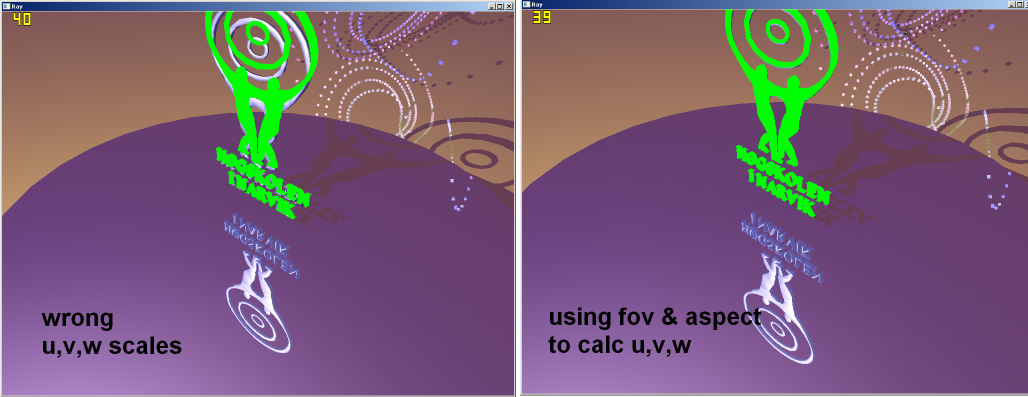
\includegraphics[width=0.90\textwidth]{Media/implementation_camera.png}
  \caption{During development, we didn't get raster and ray cameras synced on first try...}   
  \label{fig:raster_ray_camera}
\end{figure}

\paragraph{Description of the rendering pipeline}

GL and OptiX scenes are independently rendered. We end up with two sets of g-buffers, shading and composition is done in a shader.

\subsection{Camera model}
The raytracer uses pinhole camera model. The eye is a point, rays are cast from this point, through the viewplane and into the scene. Eyepoint-viewplane distance determines focal length. A rasterizer on the other hand requires a projection matrix.

\subsection{Geometry}

OptiX is programmable to the level that all geometry must have its own program. Even triangle geometry. Sadly, the acceleration structures are not programmable. The KD-tree and Split-BVH acceleration structures expect the vertex format to be packed (3 floats for position followed by 3 for normal and so on). In our code, we found it useful to keep data seperate (list all data for positions, followed by normals), but this limited us to using the BVH acceleration structure only. The reason for using this, is that optional vertex data (for example tangents) can be ommitted. One doesn't need to create a vertex format for every combination.

\lstinputlisting[language=C++,caption={OptiX Triangle Intersection program},label=triangle_mesh_small.cu]{6_Implementation/trimesh.cu}

Notice how normals in \autoref{triangle_mesh_small.cu} are read by supplying a normal offset variable, and adding it to the vertex position index.